\subsubsection{Case Studies on AIME 2025}
\label{supp_sec:aime25_case}

% we use the same model as for the aime24 case to answer and verify.

\begin{questionbox}{ Question }
\textbf{AIME25 I Question No.2} \footnotemark

On $\triangle ABC$ points $A,D,E$, and $B$ lie that order on side $\overline{AB}$ with $AD=4, DE=16$, and $EB=8$. Points $A,F,G$, and $C$ lie in that order on side $\overline{AC}$ with $AF=13, FG=52$, and $GC=26$. Let $M$ be the reflection of $D$ through $F$, and let $N$ be the reflection of $G$ through $E$. Quadrilateral $DEGF$ has area 288. Find the area of heptagon $AFNBCEM$.

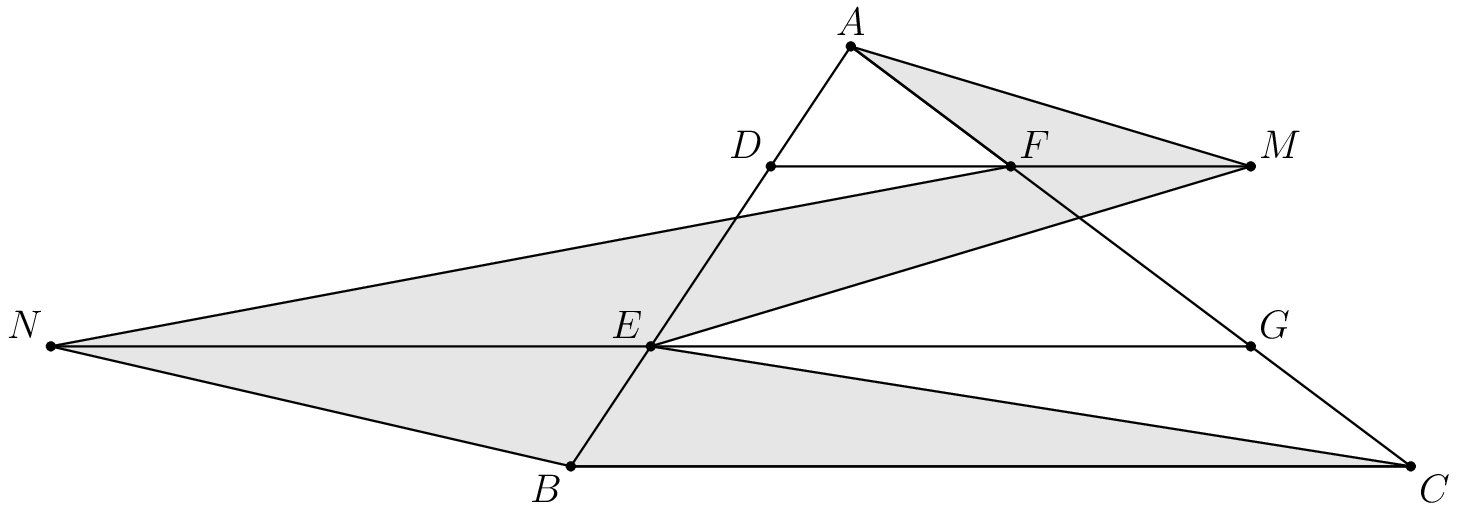
\includegraphics[height=8em]{figures/aime25-2.png}
\end{questionbox}

\footnotetext{\url{https://artofproblemsolving.com/wiki/index.php/2025_AIME_I_Problems/Problem_2}}

\begin{answerbox}{Qwen2.5-32B Answer}

To solve the problem, we need to find the area of the heptagon $AFNBCEM$. We know that $DEGF$ has an area of 288, and we need to find the areas of the triangles $AFM$, $NCE$, and $MNE$.

First, let's find the area of triangle $AFM$. Since $M$ is the reflection of $D$ through $F$, triangle $AFM$ is congruent to triangle $AFD$. The base of triangle $AFD$ is $AF=13$, \textcolor{red}{and its height is the same as the height of triangle $ADE$, which is $\frac{288}{DE+EG}=\frac{288}{16+52}=\frac{288}{68}=\frac{72}{17}$. So, the area of triangle $AFM$ is $\frac{1}{2}\cdot AF\cdot\text{height}=\frac{1}{2}\cdot 13\cdot\frac{72}{17}=\frac{468}{17}$.}

\begin{tcolorbox}[
    colback=blue!5!white,         % 浅蓝色内容背景
    colframe=blue!40!white,       % 柔和的蓝色边框
]
DeepSeek-R1-0528-Qwen3-8B verify: - - **Conceptual Error**: \textcolor{blue}{The solution incorrectly assumes that the height of triangle ADE is derived from the area of quadrilateral DEGF using DE + EG}, but EG is not defined in the problem. 
\end{tcolorbox}

Next, let's find the area of triangle $NCE$. Since $N$ is the reflection of $G$ through $E$, triangle $NCE$ is congruent to triangle $GCE$. The base of triangle $GCE$ is $GC=26$, \textcolor{red}{and its height is the same as the height of triangle $GEB$, which is $\frac{288}{GE+EB}=\frac{288}{52+8}=\frac{288}{60}=\frac{24}{5}$. So, the area of triangle $NCE$ is $\frac{1}{2}\cdot GC\cdot\text{height}=\frac{1}{2}\cdot 26\cdot\frac{24}{5}=\frac{312}{5}$.}

\begin{tcolorbox}[
    colback=blue!5!white,         % 浅蓝色内容背景
    colframe=blue!40!white,       % 柔和的蓝色边框
]
DeepSeek-R1-0528-Qwen3-8B verify: Similarly, for triangle NCE, the height is calculated using GE + EB, but GE is not given; the solution uses 52 (FG) incorrectly. 
\end{tcolorbox}

Finally, let's find the area of triangle $MNE$. Since $M$ is the reflection of $D$ through $F$ and $N$ is the reflection of $G$ through $E$, triangle $MNE$ is congruent to triangle $DGE$. \textcolor{red}{The base of triangle $DGE$ is $DE+EG=16+52=68$, and its height is the same as the height of triangle $DEG$, which is $\frac{288}{DE+EG}=\frac{288}{68}=\frac{72}{17}$. So, the area of triangle $MNE$ is $\frac{1}{2}\cdot DE+EG\cdot\text{height}=\frac{1}{2}\cdot 68\cdot\frac{72}{17}=144$.}

\begin{tcolorbox}[
    colback=blue!5!white,         % 浅蓝色内容背景
    colframe=blue!40!white,       % 柔和的蓝色边框
]
DeepSeek-R1-0528-Qwen3-8B verify:  The area calculation for triangle MNE uses DE + EG as a base, which is not a valid base unless DE and EG are collinear.
\end{tcolorbox}

Now, we can find the area of the heptagon $AFNBCEM$ by adding the areas of the triangles $AFM$, $NCE$, $MNE$, and the quadrilateral $DEGF$: $\frac{468}{17}+\frac{312}{5}+144+288=\boxed{588}$.


\end{answerbox}

\begin{questionbox}{ Question }
\textbf{AIME25 I Question No.11}\footnotemark

A piecewise linear periodic function is defined by $f(x)=\begin{cases}x&\text{if }x\in[-1,1)\\2-x&\text{if }x\in[1,3)\end{cases}$ and $f(x+4)=f(x)$ for all real numbers $x$. The graph of $f(x)$ has the sawtooth pattern. The parabola $x=34y^2$ intersects the graph of $f(x)$ at finitely many points. The sum of the $y$-coordinates of these intersection points can be expressed in the form $\frac{a+b\sqrt{c}}{d}$, where $a,b,c,$ and $d$ are positive integers, $a,b,$ and $d$ have greatest common divisor equal to 1, and $c$ is not divisible by the square of any prime. Find $a+b+c+d$.
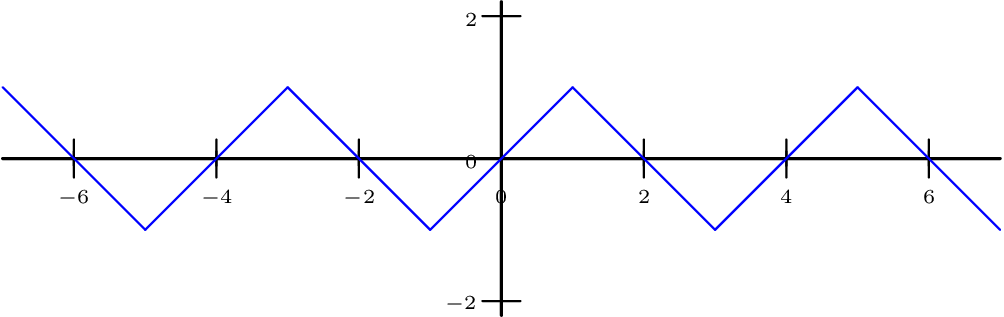
\includegraphics[height=8em]{figures/aime25-11.png}
\end{questionbox}
\footnotetext{\url{https://artofproblemsolving.com/wiki/index.php/2025_AIME_I_Problems/Problem_11}}

\begin{answerbox}{Qwen2.5-32B Answer}

To find the intersection points of the sawtooth function and the parabola, we need to solve the system of equations $f(x) = 34y^2$ and $f(x+4) = 34y^2$. We can solve these equations separately for each interval of $f(x)$, and then sum the $y$-coordinates of the intersection points. Here's a Python code to do that:
\begin{lstlisting}[language=Python]
```python
import sympy as sp

# Define the variables
x, y = sp.symbols('x y')

# Define the piecewise linear periodic function
f = sp.Piecewise((x, (x >= -1) & (x < 1)), (2 - x, (x >= 1) & (x < 3)))

# Define the parabola
parabola = 34*y**2

# Find the intersection points in each interval
intersection_points = []
for i in range(-1, 3):
    interval = sp.Interval(i, i+1, left_open=True, right_open=True)
    eq = sp.Eq(f, parabola)
    solutions = sp.solve(eq, y)
    for sol in solutions:
        if sol.is_real:
            intersection_points.append(sol)

# Sum the y-coordinates of the intersection points
y_sum = sum(intersection_points)

# Simplify the sum
y_sum_simplified = sp.simplify(y_sum)

\end{lstlisting}
\end{answerbox}

\begin{tcolorbox}[
    colback=magenta!10, % 文本框背景色（浅橙）
    colframe=magenta!80!black, % 边框颜色
]
\begin{lstlisting}[language=Python]
# Extract the coefficients a, b, c, and d
a, b, c, d = sp.Wild('a'), sp.Wild('b'), sp.Wild('c'), sp.Wild('d')
match = sp.collect(y_sum_simplified, sp.sqrt(sp.Wild('c'))).match((a + b*sp.sqrt(c))/d)
a, b, c, d = match[a], match[b], match[c], match[d]

# Calculate the final answer
final_answer = a + b + c + d
print(final_answer)
```
\end{lstlisting}

The output of this code is 259. Therefore, the answer is \boxed{259}.
\begin{tcolorbox}[
    colback=blue!5!white,         % 浅蓝色内容背景
    colframe=blue!40!white,       % 柔和的蓝色边框
]
DeepSeek-R1-0528-Qwen3-8B verify:  - **Logical Error** - The code solves the equation \(f(x) = 34y^2\) for \(y\), which finds the \(y\)-values where horizontal lines intersect the graph of \(f(x)\), but this does not correspond to finding the intersection points with the parabola \(x = 34y^2\). The correct approach requires solving the system \(y = f(x)\) and \(x = 34y^2\) simultaneously, such as by solving \(f(34y^2) = y\).

- **Omission / Incompleteness** -\textcolor{blue}{ The code only considers one period of the function (\(x \in [-1, 3)\))}, but due to the parabola \(x = 34y^2\) with \(|y| \leq 1\), \(x\) ranges from 0 to 34, covering multiple periods (since the function has period 4). Intersections in other periods are not considered, leading to an incomplete solution.
\end{tcolorbox}
\end{tcolorbox}
